

\begin{table*}[t]
\centering
\small
\setlength{\tabcolsep}{5pt}
\renewcommand{\arraystretch}{1.18}
\begin{tabular}{l c c c c c c c c}
\toprule
\multirow{2}{*}{\textbf{Model}} &
\multirow{2}{*}{\textbf{Op-count \(g\)}} &
\multirow{2}{*}{\textbf{\# Jobs}} &
\multicolumn{3}{c}{\textbf{Operator-count grouping}} &
\multicolumn{3}{c}{\textbf{Prover-time-aware grouping}} \\
\cmidrule(lr){4-6}
\cmidrule(lr){7-9}
&
&
&
\textbf{Agg. time} &
\textbf{Max time} &
\textbf{Peak mem.} &
\textbf{Agg. time} &
\textbf{Max time} &
\textbf{Peak mem.} \\
\midrule

\multirow{5}{*}{MobileNetV2}
  & 1       & 98  & 5362 s & 455 s  & 45.3 GB  & --      & --     & -- \\
  & 2       & 49  & 6241 s          & 733 s  & 55.6 GB  & 7257 s  & 988 s  & 86.5 GB \\
  & 4       & 25  & 6872 s          & 1034 s & 75.9 GB  & 7925 s  & 1254 s & 137.3 GB \\
  & 8       & 13  & 7458 s          & 1739 s & 148.2 GB & 8266 s  & 1838 s & 308.8 GB \\
  & $|V|$   & 1   & 7858 s          & 7858 s & 587.6 GB & --      & --     & -- \\
\midrule

\multirow{5}{*}{NanoGPT (4L)}
  & 1       & 192 & 775 s  & 46 s   & 7.8 GB   & --      & --     & -- \\
  & 2       & 96  & 882 s           & 68 s   & 13.2 GB  & 1004 s  & 78 s   & 17.2 GB \\
  & 4       & 48  & 930 s           & 86 s   & 14.6 GB  & 1230 s  & 138 s  & 19.4 GB \\
  & 8       & 24  & 1425 s          & 157 s  & 25.7 GB  & 1555 s  & 221 s  & 28.7 GB \\
  & $|V|$   & 1   & 4068 s          & 4068 s & 556.4 GB & --      & --     & -- \\
\bottomrule
\end{tabular}
\caption{
Model-splitting characterization results. Each row reports the number of proving jobs and, for each splitting policy, aggregate prover time, maximum job time, and maximum peak memory across jobs. Rows with \(g=|V|\) correspond to full-model proving. Dashes indicate cases where the two policies coincide. Lower values are better.
}
\label{tab:model-splitting-results}
\end{table*}

 

\section{Characterizing Proving Granularity}
\label{sec:proof-splitting}
We characterize proving granularity by varying the amount of model computation assigned to each proving job. The coarsest configuration places the entire ONNX graph in a single job, while the finest creates one job per operator. Intermediate configurations group consecutive operators into jobs of varying sizes. We evaluate how these choices affect proving time, peak memory, job heterogeneity, and the parallelism available to the serving system.

\subsection{Characterization Setup}

\noindent\textbf{Workloads and setup.}
The characterization uses two workloads from the model suite summarized in Table~\ref{tab:models}. MobileNetV2 is a depthwise-separable convolutional network, while NanoGPT is a GPT-style decoder-only transformer. We choose these models because they come from different architecture families and lead to different ONNX graph structures. All measurements use EZKL's Halo2-based proving pipeline~\cite{ezkl} on a dedicated CPU server with two AMD EPYC 9354 processors and 768~GB of RAM.

\noindent\textbf{Splitting policies.}
We evaluate two policies for partitioning the ONNX computation graph into
proving jobs. Both policies arrange the executable ONNX operators (i.e.,
operators that perform computation at inference time) in topological order
and divide the resulting sequence into consecutive groups, each forming one
proving job. 
% This preserves the graph's execution dependencies while keeping
% the characterization focused on proving granularity rather than general
% graph-partitioning heuristics.
\begin{enumerate}
    \item \textit{Operator-count grouping.}
    Let \(V\) denote the set of executable operators. Given a group size
    \(g\), this policy divides the topological order into consecutive groups
    of at most \(g\) operators. Thus, \(g=1\) corresponds to operator-level
    proving.
    \item \textit{Prover-time-aware grouping.}
    This policy produces the same number of jobs as operator-count grouping
    for a given \(g\), but uses profiling information to place the split
    points. We first profile each executable operator \(v \in V\) once,
    recording the time \(t_v\) required to prove it independently. We then
    choose split points along the topological order so as to minimize the
    maximum estimated job cost, where the cost of a job is the sum of the
    profiled times \(t_v\) of its operators.
\end{enumerate}
For each workload, we evaluate group sizes \(g \in \{1,2,4,8\}\), omitting
values larger than \(|V|\), and include a full-model baseline in which the
entire graph forms a single proving job (\(g = |V|\)).



\noindent\textbf{Metrics.}
For each splitting configuration, we execute the resulting proving jobs sequentially and report three metrics. \textit{Aggregate time} is the total prover time across all jobs. \textit{Max job time} is the longest prover time of any individual job. \textit{Peak memory} is the largest per-job memory footprint and determines the minimum memory capacity required to execute the configuration. Prover time includes witness generation and proof construction, but excludes offline setup costs such as circuit compilation and the generation of proving and verification keys.
\subsection{Effect of Proving Granularity}

Table~\ref{tab:model-splitting-results} presents the
results. We highlight four findings.

\noindent\textbf{Finding 1. Partitioning reduces aggregate prover time.}
Splitting a model into smaller jobs reduces the aggregate prover time in
addition to exposing parallelism. Proving NanoGPT at operator granularity
takes \(\qty[quantity-product = {}]{775}{\second}\) in total, compared to
\(\qty[quantity-product = {}]{4068}{\second}\) for the full model, a
\(\num{5.2}\times\) reduction.
MobileNetV2 shows a similar but smaller reduction, from
\(\qty[quantity-product = {}]{7858}{\second}\) to
\(\qty[quantity-product = {}]{5362}{\second}\). For both models,
aggregate time decreases steadily as jobs become finer grained.







% Intermediate
% granularities can thus be more expensive than either extreme.

\noindent\textbf{Finding 2. Fine granularity sharply reduces the longest
job.}
Max job time falls from
\(\qty[quantity-product = {}]{7858}{\second}\) to
\(\qty[quantity-product = {}]{455}{\second}\) for MobileNetV2 and from
\(\qty[quantity-product = {}]{4068}{\second}\) to
\(\qty[quantity-product = {}]{46}{\second}\) for NanoGPT when moving from
full-model to operator-level proving, corresponding to
\(\num{17}\times\) and \(\num{88}\times\) reductions, respectively.
Since max job time lower-bounds end-to-end latency under parallel
execution, finer granularity directly reduces the minimum achievable
proving latency. 





\noindent\textbf{Finding 3. Memory makes full-model proving impractical.}
Full-model proving reaches peak memory footprints of
\(\qty[quantity-product = {}]{587.6}{\giga\byte}\) for MobileNetV2 and
\(\qty[quantity-product = {}]{556.4}{\giga\byte}\) for NanoGPT, requiring
high-memory servers and consuming much of the
\(\qty[quantity-product = {}]{768}{\giga\byte}\) available on our evaluation
machine. Operator-level proving reduces peak memory to
\(\qty[quantity-product = {}]{45.3}{\giga\byte}\) and
\(\qty[quantity-product = {}]{7.8}{\giga\byte}\), respectively,
substantially broadening the range of machines capable of executing an
individual proving job. Since the largest job determines the minimum memory
capacity required of a worker, proving granularity directly affects the class
of hardware on which proof generation can run.



\noindent\textbf{Finding 4. Standalone operator profiles do not predict grouped proving cost.}
Prover-time-aware grouping is intended to equalize job costs, yet it
increases maximum job time in every evaluated configuration. For example,
at \(g=2\), maximum job time for MobileNetV2 increases from
\(\qty[quantity-product = {}]{733}{\second}\) to
\(\qty[quantity-product = {}]{988}{\second}\), while peak memory increases
by up to \(\num{2.1}\times\). These results indicate that the sum of
standalone operator times does not reliably predict the cost of proving
those operators together in a single job. Split decisions therefore should
not rely only on summed operator-level profiles.



% \subsection{Effect of Proving Granularity}
% Table~\ref{tab:model-splitting-results} shows that fine-grained model splitting substantially reduces prover cost relative to full-model proving. With operator-level proving, \(g=1\), aggregate prover time improves by \(1.5\times\) for MobileNetV2 and \(5.2\times\) for NanoGPT. Peak memory falls even more sharply, by \(13.0\times\) and \(71.3\times\), respectively. The maximum job time also drops, since each prover invocation handles only a small portion of the original computation. As \(g\) increases, the per-job benefits diminish because larger groups place more operators in each proving job, increasing both the longest job time and the per-job memory footprint. These results motivate fine-grained operator-count grouping as a simple and effective splitting strategy. It requires only the ordered ONNX graph, does not depend on prior profiling runs, and achieves the best aggregate time and peak memory for both workloads at \(g=1\). The prover-time-aware policy provides little additional benefit over this baseline. For MobileNetV2, it slightly reduces aggregate time at some intermediate group sizes, but increases peak memory and does not reduce maximum job time. For NanoGPT, it is worse than operator-count grouping across the intermediate group sizes. This suggests that, for these workloads, the main benefit comes from fine-grained proving rather than profiling-based split placement. We use this result to guide the default splitting policy in \TITLE{}.





\begin{figure}[t]
\centering
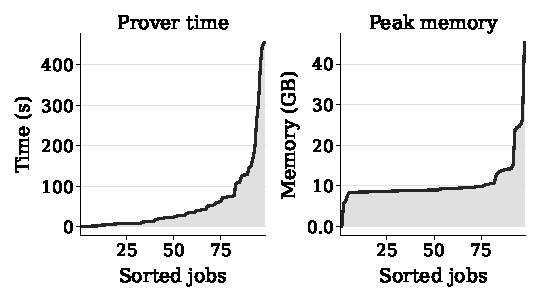
\includegraphics[width=\columnwidth]{figures/characterization/mobilenetv2_g1_sorted_job_tail.pdf}
\caption{Heterogeneity across MobileNetV2 operator-level proving jobs. Jobs are ordered independently by increasing prover time in the \textit{Prover Time} panel and increasing peak memory in the \textit{Peak Memory} panel.
}
\label{fig:operator-job-tail}
\end{figure}

\subsection{Systems Challenges of Fine-Grained Proving}
Although operator-level splitting achieves the lowest overall proving
cost in Table~\ref{tab:model-splitting-results}, it produces jobs with
widely varying execution times and memory requirements. Figure~\ref{fig:operator-job-tail} shows per-job prover time and
peak memory for MobileNetV2 at \(g=1\).  Most jobs are inexpensive, while a small number take much
longer or consume substantially more memory. These differences become
important when many jobs run concurrently. A request finishes only after
all of its jobs complete, so delaying an expensive job can
increase end-to-end latency even if the remaining jobs finish quickly.
Memory demand further limits which workers can execute a job, since each
worker must have enough available memory to accommodate the job's peak
usage. A scheduler must therefore consider both expected proving time
and memory demand when deciding which job to run next and which worker
should execute it.

Fine-grained splitting also changes how intermediate activations are
managed. In a full-model proof, all intermediate values remain internal
to a single prover invocation and are incorporated into one witness.
After splitting, values that cross partition boundaries must be made
available to the corresponding proving jobs as request-specific inputs.
The execution system must therefore identify these boundary values,
associate them with the jobs that consume them, and preserve their
consistency across independently generated proofs. Without this support,
the partitions defined by the splitting policy cannot be executed as
independent proving jobs.


The larger number of prover invocations also makes reuse of setup
artifacts essential. Each job relies on a compiled circuit and a
corresponding proving key. These artifacts are expensive to generate, but
they can be reused across requests that share the same model and
splitting configuration. Rebuilding them for every request would add
substantial unnecessary overhead and could outweigh the savings obtained
from smaller proofs.

Supporting fine-grained proving therefore requires an execution system
that accounts for differences in job cost, supplies each job with the
request-specific values needed to construct its witness, and reuses
proving artifacts across requests.

proving, intermediate activations remain internal to one backend invocation. After splitting, these values become boundaries between proof jobs. A downstream job cannot run until the tensors produced by its predecessors are available, and those tensors must be materialized, stored, and supplied to the worker that executes the downstream job. The runtime must therefore manage intermediate tensors as part of execution rather than treating each proof job as an isolated backend call.


\label{sec-partition-characterization-results}